

\section{Background}
\subsection{API Remoting}
Scheduling the potentially multiple GPUs in future manycore platforms demands (i) the logical aggregation of all GPUs to make them visible to the scheduler and then (ii) decoupling the CPU-GPU association programmed into a GPU-based application. Previous work (e.g., GVim~\cite{gvim}, vCuda~\cite{vcuda}, rCuda~\cite{rcuda}, Pegasus~\cite{pegasus}, gVirtus~\cite{gvirtus}) adopts an API-driven separation of an application’s CPU from its GPU components. As shown in Figure~\ref{fig:remoting}a. , (i) a frontend implemented as a CUDA runtime interposer library dynamically links with the application, responsible for intercepting the CUDA runtime API calls, and (ii) a backend is realized as a daemon responsible for receiving GPU requests from the frontend, dispatching the CUDA runtime library calls to the attached GPUs, and returning error codes and/or output parameters to the frontend. A useful side effect of this architecture is the ability to execute an application’s GPU component on a GPU attached to some remote node, termed \textit{API Remoting}. We can use it to create an emulated high-end multi-GPU server machine with more GPUs than those available on today’s single physical platforms. Specifically, for such multi-GPU servers, we can aggregate all GPUs into a single logical pool, termed a gPool, for use by the GPU scheduler. Figure~\ref{fig:remoting}b. shows the logical transformation of a small-scale cluster machine with per-node GPUs into a set of GPUs schedulable via a shared GPU pool.

\subsection{Gather-Apply-Scatter Model}
With Gather-Apply-Scatter (GAS) computational model used by Pregel \cite{pregel}, Powergraph \cite{powergraph}, and GraphLab \cite{graphlab}, a problem is described as a directed (sparse) graph, $G = (V, E)$, where $V$ denotes the vertex set and $E$ denotes 
the directed edge set. A value is associated with each vertex $v\in V$, and each directed edge $e_{ij}$ is associated with 
a source vertex $u$ and a target vertex $v$: $e_{ij} =(u, v) \in E$. Given a directed edge $e_{ij} = (u, v)$, we refer to 
$e_{ij}$ as vertex $v$'s in-edge, and as vertex $u$'s out-edge. A typical GAS computation, then, has three stages \cite{vertexapi}: 
(1) Initialization, (2) Iterations, and (3) Output. Initialization deals with initializing vertex/edge values and a starting 
{\em computation frontier}, which is defined as the set of active vertices for a given iteration. In each Iteration stage, 
a sequence of iterations is run, each gathering the values seen on incoming edges, updating the values of elements, and 
then defining a new frontier for the next iteration. Figure~\ref{fig:design}a. illustrates these three phases, assuming vertex $v$ to be the 
central vertex.


\vspace{-0.5\baselineskip}
\begin{itemize}
  \item {\bf Gather Phase}: each vertex aggregates values associated with its incoming edges and their source vertices. 
We define the gather function as $G(u, v, e_{ij})$, and we use binary operator $\biguplus$ to aggregate the outputs 
from multiple $G$s into one value $R$. As shown in the figure, the result ($R$) from the Gather Phase for vertex $v$ can be represented 
as $R= G(u_1, v, a)\biguplus G(u_2, v, b)$. 
  \vspace{-0.5\baselineskip}
  \item {\bf Apply Phase}: the value of each vertex in the current frontier is updated through the gather result. 
We define the update function as $U(v, R)$, where $R$ is the result from the Gather Phase. Here 
we have the updated vertex $v$ as: $v' = U(v, R)$.  
  \vspace{-0.5\baselineskip}
  \item {\bf Scatter Phase}: the new vertex state is propagated to neighbors, by updating the state of its out-edges 
(e.g., $c$ and $d$ in the figure). We define the Scatter function for updating the out-edges of $v$ as $S(v', e_{out})$, 
where $v'$ is the updated vertex $v$ and $e_{out}$ represents $v$'s out-edges. Here, two updated edges 
$c'$ and $d'$ are denoted as: $c' = S(v', c)$ and $d' = S(v', d)$.
\vspace{-0.5\baselineskip}
\end{itemize} 


As shown in much prior work \cite{powergraph, pregel}, the GAS model is not only simple to use, but it is also sufficiently general to express
a broad set of graph algorithms, ranging from PageRank to Connected Components, and from Heat Simulation to Sparse Linear Algebra. 
For example, the PageRank algorithm \cite{pagerank} can be expressed as follows. In the {\bf Gather Phase}, each vertex $v_i$ in the current 
frontier accumulates $G_i = \sum_{}^{}{\frac{R_j}{n_j}}$ from all in-edges from source vertex $v_j$, where $R_j$ is the rank of 
$v_j$ and $n_j$ is the number of out-edges ($v_j\rightarrow v_i$) of $v_j$. Then, in the {\bf Apply Phase}, vertex $v_i$ updates 
its value using some common PageRank formula like $R_i = 0.85+0.15\times G_i$. Since in PageRank, the value of $v_i$ will not change 
in the {\bf Scatter Phase}, there are no operations for this phase. 

\begin{center}
\begin{figure*}[t]
\begin{center}
\begin{minipage}{0.49\textwidth}
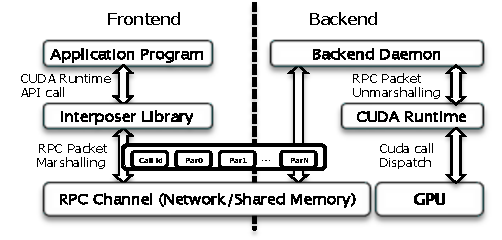
\includegraphics[width=\textwidth, height=4cm]{GPU-remoting}
\end{minipage}
\begin{minipage}{0.49\textwidth}
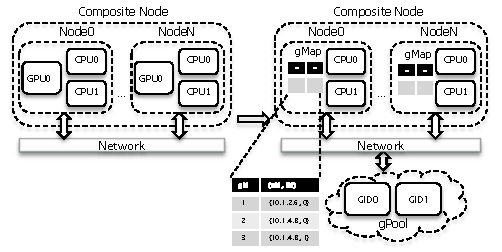
\includegraphics[width=\textwidth, height=4cm]{GPool}
\end{minipage}
\caption{\small a) Architecture of API	 Remoting. b) Logical transformatiom of GPU cluster after gPool creation.}
\label{fig:remoting}
\end{center}	
\end{figure*}
\end{center}

\label{fig:prob}
\begin{center}
\begin{figure*}[t]
\begin{center}
\begin{minipage}{0.49\textwidth}
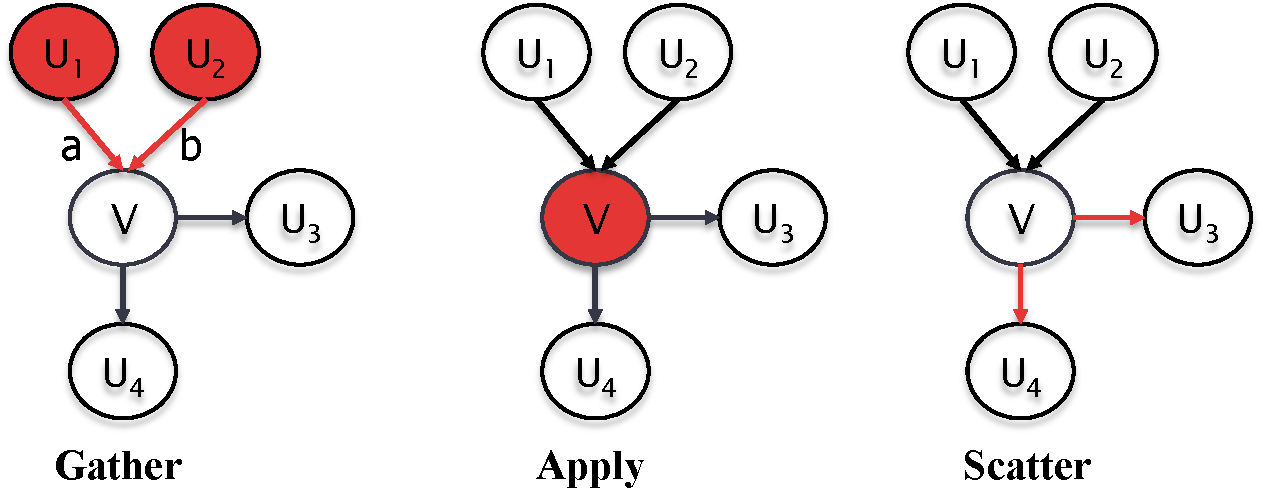
\includegraphics[width=\textwidth]{GAS}
\end{minipage}
\begin{minipage}{0.49\textwidth}
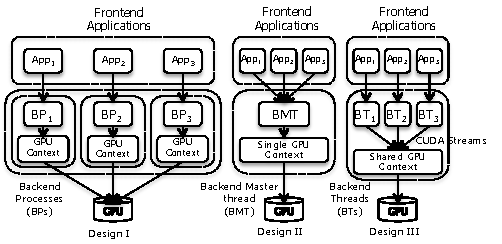
\includegraphics[width=\textwidth]{Strings-design}
\end{minipage}
\caption{\small a) An example of GAS abstraction. b) Three different implementations GPU remoting.}
\label{fig:design}
\end{center}	
\end{figure*}
\end{center}
